\section{Introduction to Electric Potential}
\label{potential_intro}
\begin{comment}
This lab was written by Matt Trawick in December, 2016.  It is intended to be a first introduction to the idea of V, and relating E and V.  
I intend for this to take the place of the first part of the lab on electric potential from Dickinson College.  That lab does a lot of things well, and I intend to recycle some of the material from there in future labs.
\end{comment}


\makelabheader %(Space for student name, etc., defined in master.tex)

\bigskip

\textbf{Introduction} 

In this lab, we'll start by reviewing the ideas of force, work, and potential energy from physics 131.  Then we'll define a new, handy quantity called the ``electric potential'' that's one of the key ideas in physics 132.

\bigskip

\textbf{Activity 0: Review of Force and Potential Energy from Physics 131}\footnote{This activity could be done as homework before the rest of the lab.}

In your previous physics class, you learned that the work $W$ done on an object by a uniform force $F$ is given by $W=\vv{F} \cdot \vv{{\scriptstyle \Delta} s}$, where $\vv{{\scriptstyle \Delta} s}$ is the displacement of the object.

\begin{enumerate}[labparts]

\item Suppose that a ball moves along each of the four numbered paths shown below.  For each one, is the work done by the force of gravity \textit{positive}, \textit{negative}, or \textit{zero}? \label{part_potential_intro_grav_work} 
\begin{center}
\vspace{0.1in}
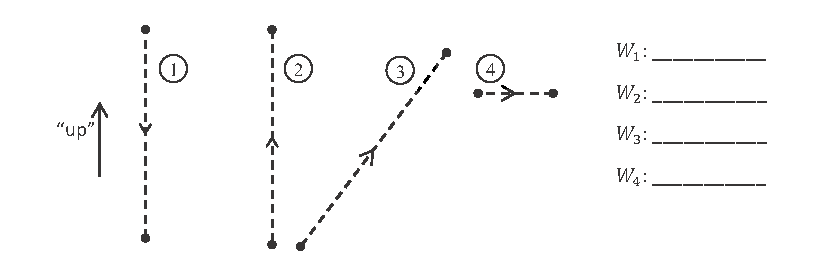
\includegraphics{potential_intro/activity_1_figs/gravity_paths.eps}
\vspace{0.1in}
\end{center}

For forces like gravity that only depend on the position of the object, you learned that instead of treating the force as  ``external'' (from outside the system) it's sometimes handy to include the source of the force (the Earth, in this case) as a part of the system, defining a potential energy $U$ so that
$$\Delta U \equiv -W.$$

\item For each of the four paths in the figure in part \ref{part_potential_intro_grav_work}, state whether the change in gravitational potential energy $\Delta U$ of the system is \textit{positive}, \textit{negative}, or \textit{zero}.
\begin{center}
\vspace{0.05in}

\includegraphics{potential_intro/activity_1_figs/gravity_potentials.eps}
\vspace{0.05in}
\end{center}

\textit{Helpful hint: It's easy to make a careless algebraic mistake with a sign, so always check yourself by telling yourself a little story like this: if you were to reach into the system with your hand and lift a ball along path 2, the external force of your hand would be doing \textit{positive} work on the system---that's why you get tired.  The calories you burned went someplace, and they went to \textit{increasing} the gravitational potential energy of the system. }

\pagebreak[3]

\item For non-uniform forces (that is, forces that change with position), the work done by a force is given by 
$$W=\int{\vv{F} \cdot \vv{ds}}$$
which reduces to just $W=\int{F ds}$ in one dimension.  The diagram below shows the resulting general relationship between force $\vv{F}$ and potential energy $U$.  Complete the equation on the right showing how to find the force if you know the potential energy $U$.  (Yep, it'll be the opposite of an integral.)
\begin{center}
\vspace{-0.1in}
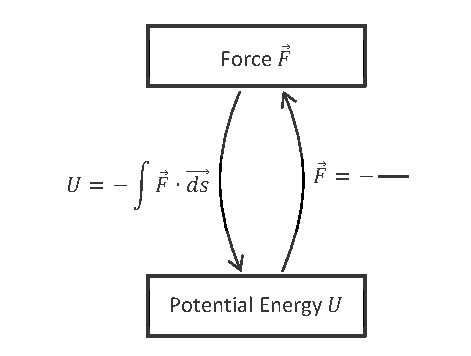
\includegraphics{potential_intro/concept_map_figs/concept_map_F_and_U_blank_squish.eps}
\end{center}

%\end{enumerate}

%\begin{minipage}{0.64\textwidth}
%\begin{enumerate}[resume,wide, label=(\emph{\alph*})]
\item As an example, consider a mass $m$ on a spring with a spring constant $k$ in the figure to the right.  For simplicity, we'll assume the surface is frictionless, and that the equilibrium position of the mass is at $x=0$.  
Draw a graph of the force $F$ of the spring on the mass, as a function of its position $x$.  
(Hints: this is your old friend, Hooke's law.  Also, think about the signs: if the mass is at a positive $x$, is the force of the spring pushing it in the positive direction or the negative direction?)
%\end{enumerate}
%\end{minipage}
%\begin{minipage}{0.34\textwidth}
%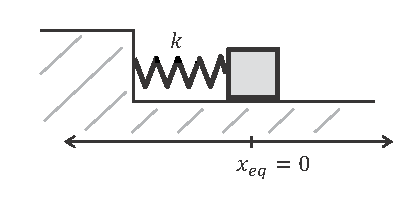
\includegraphics[width=1.0\textwidth]{potential_intro/activity_1_figs/mass_on_spring.eps}
%\end{minipage}

\begin{center}
%\vspace{-0.1in}
%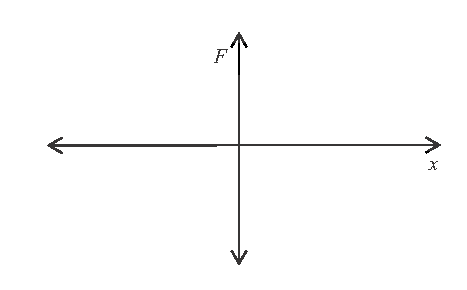
\includegraphics{potential_intro/activity_1_figs/F_axes.eps}
\begin{lab_axis}[lab_noticks_4quads,
	width={3.0in}, height={1.7in},
	xlabel={$x$},
	ylabel={$F$},
	]
\end{lab_axis}
\hspace{0.5in}
\raisebox{0.3in}{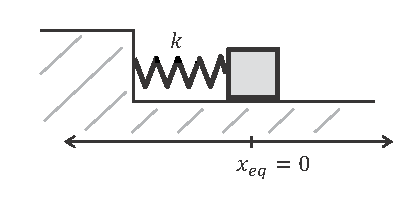
\includegraphics[scale=0.8]{potential_intro/activity_1_figs/mass_on_spring.eps}}
\end{center}

%\begin{enumerate}[resume*,start=5] %this hard-codes the start at letter e.  Somehow it always restarted at d before.

%\newpage

\item From the force law $F(x)$ you just graphed, write an expression $U(x)$ for the potential energy of the system as a function of the position of the mass.  Sketch a graph of $U(x)$ on the axes below.
\begin{center}
%\vspace{-0.1in}
%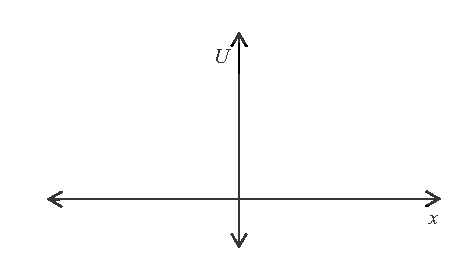
\includegraphics{potential_intro/activity_1_figs/U_axes.eps}
\begin{lab_axis}[lab_noticks_4quads,
	width={3.0in}, height={1.5in},
	xlabel={$x$},
	ylabel={$U$},
	ymin=-0.3,
	]
\end{lab_axis}
\hspace{1.05in}
\raisebox{0.3in}{$U(x)=$}
\hspace*{1.0in}
\end{center}

Note that when you integrate $F(x)$, you should include an integration constant $+C$.  It doesn't matter what you pick for $C$; you can add any constant you want to $U(x)$, because we only ever care about \textit{differences} $\Delta U$ anyway.  (It's the same as how you can define gravitational potential energy so that $U_{\rm grav}=0$ is at sea level or the top of your lab table.)  The easiest choice here is probably $C=0$.
\end{enumerate}

\pagebreak[2]
\textbf{Activity 1: Electric Potential Energy}

Now that we've reviewed gravitational potential energy $U_{\rm grav}$ and the potential energy of a spring $U_{\rm spring}$, let's take a look at an example of electric potential energy.  

\begin{enumerate}[labparts]

\item The figure below shows a region of uniform electric field $E_0$.  If a \textit{positively} charged particle $+q$ moves along the path shown with the dashed line, is the change in potential energy of the system \textit{positive}, \textit{negative}, or \textit{zero?}  Compare with the gravitational example on page \pageref{part_potential_intro_grav_work}.
\begin{center}
%\vspace{0.1in}
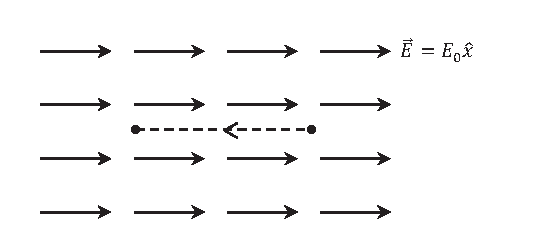
\includegraphics{potential_intro/activity_2_figs/uniform_E_field.eps}
%\vspace{0.1in}
\end{center}


\item What is the magnitude of the electric force $\vv{F}$ on the charged particle?
\answerspace{0.3in}

\item By integrating the force above, write a function for the potential energy $U(x)$ for the particle in the field.  Be sure to include an integration constant, $+C$.
\answerspace{0.3in}

\item Suppose that the particle's initial position is at $x=0$, and we want to define the potential energy $U(x)$ so that $U=0$ at $x=0$.  What value should you choose for the integration constant $C$?
\answerspace{0.3in}

\item Sketch a qualitative graph of the potential energy function $U(x)$ you just found.
%\begin{center}
%\vspace{-0.1in}
%\includegraphics{potential_intro/activity_2_figs/U_axes_2.eps}
%\vspace{-0.1in}
%\end{center}
\begin{lab_axis}*[lab_noticks_4quads,
	width={3.0in}, height={1.7in},
	xlabel={$x$},
	ylabel={$U$},
	]
\end{lab_axis}

\item Sketch a qualitative graph of what the potential energy function $U(x)$ would look like if the particle were \textit{negatively} charged.

%\begin{center}
%\vspace{-0.1in}
%\includegraphics{potential_intro/activity_2_figs/U_axes_2.eps}
%\vspace{-0.1in}
%\end{center}
\begin{lab_axis}*[lab_noticks_4quads,
	width={3.0in}, height={1.7in},
	xlabel={$x$},
	ylabel={$U$},
	]
\end{lab_axis}

\end{enumerate}

\pagebreak[3]
\textbf{Activity 2: A First Look at Electric Potential \textit{V}}

\textbf{Why Electric Field Is Useful...}


Suppose a bunch of electric charges ($Q_1$, $Q_2$, etc.) are nailed down so they don't move.  If you take an additional charge $q$ out of your pocket and place it in a specific location, there will be an electric force on it from the nailed down charges.  You could calculate the force directly, using Coulomb's law, for instance.  
\begin{wrapfigure}[8]{r}{0.27\textwidth}
\begin{center}
\vspace{-0.3 in}
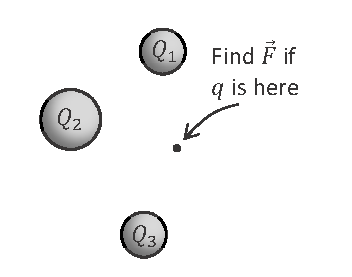
\includegraphics[scale=0.8]{potential_intro/activity_3_figs/charge_from_pocket.eps}
\end{center}
\end{wrapfigure}


But the size of the force depends on what charge $q$ you pull from your pocket, and you might not want to recalculate the force from scratch for every possible charge you could pull out.  Instead, you can calculate the electric field $\vv{E}$ due to the fixed charges, and then find the force on any charge $q$ using $\vv{F}=q\vv{E}$.  The electric field $\vv{E}$ is telling you the ``force per unit charge'' on whatever new charge $q$ you put down, and you can think of that as the definition of electric field:
$$\vv{E} \equiv \frac{\vv{F}}{q}$$
The diagram below shows the relationship between $\vv{F}$ and $\vv{E}$ graphically:

\begin{center}
\vspace{-0.1 in}
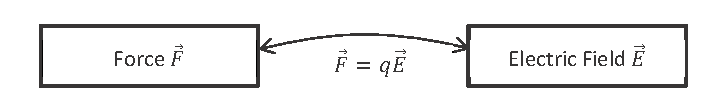
\includegraphics{potential_intro/concept_map_figs/concept_map_F_and_E.eps}
\vspace{-0.1 in}
\end{center}


\textbf{...And Why Electric Potential Is Useful Too}

%You can do the same kind of thing for electric potential energy.  
You already know how potential energy $U$ is useful for solving some problems where you only care about the initial and final states.  For example, if you know how far an object falls, you can use the change in gravitational 
potential energy to calculate its final speed.  
So what if you want to use conservation of energy to find the final 
\begin{wrapfigure}[9]{r}{0.27\textwidth}
\begin{center}
\vspace{-0.3 in}
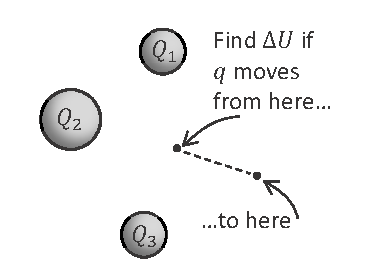
\includegraphics[scale=0.8]{potential_intro/activity_3_figs/charge_from_pocket_potential.eps}
\end{center}
\end{wrapfigure}
speed of the charge $q$ from your pocket?  You could calculate the electric potential energy at the initial and final positions, and find the change in kinetic energy using $\Delta K = -\Delta U$.

But again, the size of $\Delta U$ depends on what charge $q$ you pull from your pocket, and you might not want to recalculate it from scratch for every possible charge you could pull out.  Instead, you can calculate a new quantity called the ``electric potential'' $V$ at the initial and final positions.  Just as $E$ tells you the force per unit charge $q$, this new quantity $V$ tells you the ``potential energy per unit charge'' for whatever new charge $q$ you put down.  The electric potential is defined as:
$$V \equiv \frac{U}{q}$$
\vspace{-0.3 in}
\begin{enumerate}[labparts]

\item Go ahead and fill in the missing equation on the diagram below, analogous to the previous diagram with $\vv{F}$ and $\vv{E}$.  (It seems a little silly here, but play along anyway; the payoff is coming on the next page!)
\begin{center}
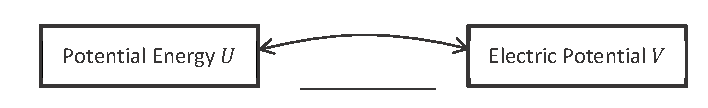
\includegraphics{potential_intro/concept_map_figs/concept_map_U_and_V_blank.eps}
\end{center}

\item Note that the name ``electric potential'' makes it sound like $V$ is an energy, but it's not.  (Even more confusing: the electric potential $V$ is sometimes called just ``the potential'' for short.)  What are the SI units for potential energy $U$?  
\answerspace{0.3in}

\item By contrast, what would be the units of electric potential $V$, in terms of SI units you already know?  (This unit is also defined as the Volt, and is abbreviated as ``V''.)
\answerspace{0.3in}

\end{enumerate}

\pagebreak[2]
\textbf{Activity 3: A Quick Example Problem}

Let's do a quick example problem to show how handy the electric potential $V$ can be.  
\begin{quote}
\textbf{Problem:} An ionized helium atom has mass $m=6.7\times 10^{-27}$~kg and charge $q_0=+1.6\times 10^{-19}$~C.  It is released from rest at a place where the electric potential is $V = 80$~Volts.  (1 Volt = 1 Joule/Coulomb.)  The ion accelerates to a final location where the electric potential is $V= 25$~Volts.  What is the final speed $v_F$ of the helium ion?  
\end{quote}
\begin{enumerate}[labparts]
\item Find the change in the electric potential $\Delta V$ for the helium ion.  (Be careful with your signs!)
\answerspace{0.3in}

\item Find the change in the helium ion's potential energy $\Delta U$.  
\answerspace{0.3in}

\item What is the change in the helium ion's kinetic energy, $\Delta K$? 
\answerspace{0.3in}

\item What is the final speed $v_F$ of the helium ion?
\answerspace{0.6in}

\end{enumerate}
\textit{Note that in this problem the electric potential at the two locations was given to you; you'll learn how to calculate $V$ on your own soon enough.}

\bigskip
\textbf{Activity 4: Relating Electric Field and Electric Potential}

The relationship between the electric field $\vv{E}$ and electric potential $V$ is exactly analogous to that between force $\vv{F}$ and potential energy $U$.  

\begin{enumerate}[labparts]

\item The diagram below shows the relationships between $\vv{F}$, $\vv{E}$, $U$, and $V$.\footnote{Technically, the exact notation $F=-\frac{dU}{ds}$ in the diagram is only applicable for the one-dimensional case.}
Fill in the equations between $\vv{F}$ and $\vv{E}$ and between $U$ and $V$ from memory if you can.  Then write the two relationships between $\vv{E}$ and $V$.  Hint: start with the analogous equations relating $\vv{F}$ and $U$, and divide both sides by $q$.  
\begin{center}
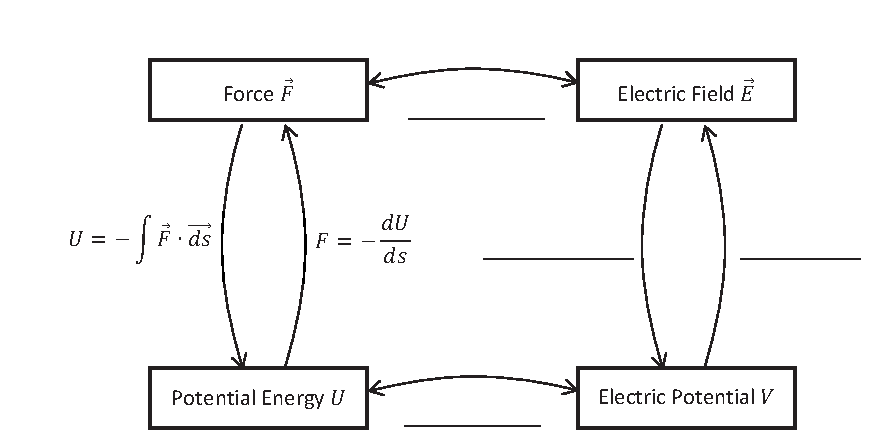
\includegraphics{potential_intro/concept_map_figs/concept_map_all_blanks.eps}
\vspace*{0.2in}
\end{center}

\item The graph below shows the electric potential $V$ along the $x$ axis.  Draw a qualitative graph showing the potential energy $U(x)$ for a \textit{positively} charged particle placed on the $x$ axis.  \label{part_potential_intro_given_V}

\begin{lab_axis}*[lab_noticks_2quads,
	width={2.7in}, height={1.6in},
	algebraic_labels,
	xlabel={$x$},
	ylabel={$V$},
	xmax={6},
	xtick={2,4},
	xticklabels = { , },
	]
\addplot coordinates {(0,0) (2,0.8) (4,0.8) (5,0) (5.5,0) };
\end{lab_axis}

\begin{lab_axis}*[lab_noticks_2quads,
	width={2.7in}, height={1.6in},
	algebraic_labels,
	xlabel={$x$},
	ylabel={$U$},
	xmax={6},
	xtick={2,4},
	xticklabels = { , },
	]
\end{lab_axis}

%\begin{center}
%%\vspace{-0.1 in}
%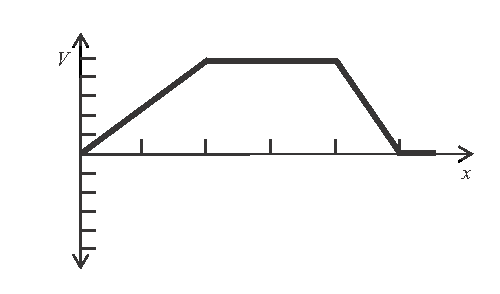
\includegraphics{potential_intro/activity_5_figs/given_V.eps}
%
%\vspace{-0.1 in}
%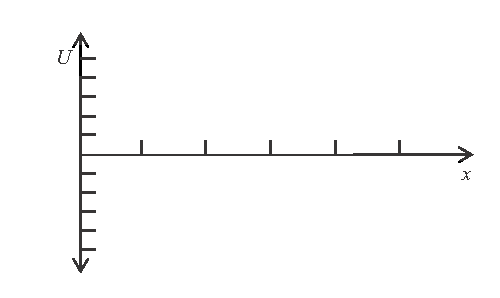
\includegraphics{potential_intro/activity_5_figs/U_axes.eps}
%%\vspace{-0.1 in}
%\end{center}

\item For the graph of $V(x)$ given in part \ref{part_potential_intro_given_V}, draw a qualitative graph showing the potential energy  $U(x)$ for an \textit{electron} placed on the $x$ axis.
%\begin{center}
%\vspace{-0.1 in}
%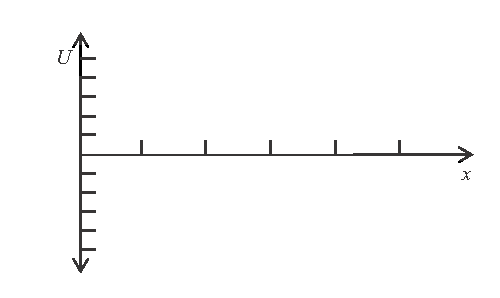
\includegraphics{potential_intro/activity_5_figs/U_axes.eps}
%%\vspace{-0.1 in}
%\end{center}
\begin{lab_axis}*[lab_noticks_2quads,
	width={2.7in}, height={1.6in},
	algebraic_labels,
	xlabel={$x$},
	ylabel={$U$},
	xmax={6},
	xtick={2,4},
	xticklabels = { , },
	]
\end{lab_axis}

%\newpage
\item  For the graph of $V(x)$ given in part \ref{part_potential_intro_given_V}, sketch a qualitative graph of $\vv{E}(x)$.
%\begin{center}
%%\vspace{-0.1 in}
%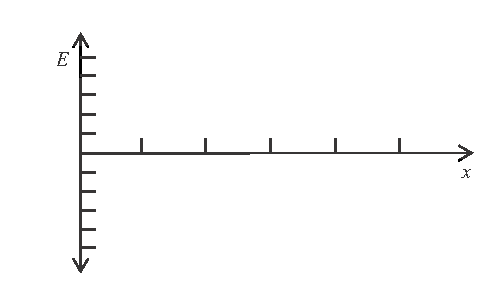
\includegraphics{potential_intro/activity_5_figs/E_axes.eps}
%%\vspace{-0.1 in}
%\end{center}

\begin{lab_axis}*[lab_noticks_2quads,
	width={2.7in}, height={1.6in},
	algebraic_labels,
	xlabel={$x$},
	ylabel={$E$},
	xmax={6},
	xtick={2,4},
	xticklabels = { , },
	]
\end{lab_axis}

\pagebreak[3]
\item The figure below shows electric field vectors in a region of space.  In traveling  along each of the dotted-line paths below, is the change in electric potential $\Delta V$ \textit{positive},  \textit{negative}, or  \textit{zero}?  (Think: if pushing a positive charge $+q$ along the path with your hand would require doing \textit{positive} work, then you would  be \textit{increasing} the potential energy of the system.)
\begin{center}
\vspace{-0.1 in}
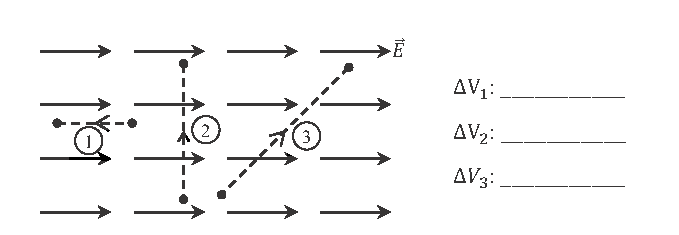
\includegraphics{potential_intro/activity_5_figs/uniform_E_field_1.eps}
\end{center}

%\item The figure below shows a region of space with a uniform electric field.  Draw two different dotted line paths, each of which has constant electric potential along the path.  Which of your two paths is at a higher electric potential?  (Each of these paths is called an ``equipotential''.)
\item  One of the three paths  above is an ``equipotential,'' meaning that every point along the path has the same electric potential $V$.  The figure below shows another region of space with a uniform electric field.  Draw two dotted line paths showing equipotentials on the figure below.  Which of your two paths is at a higher electric potential?

\begin{center}
\vspace{-0.25 in}
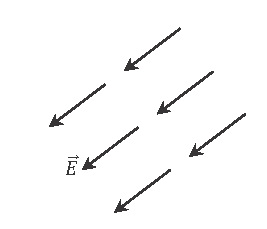
\includegraphics{potential_intro/activity_5_figs/uniform_E_field_2_squish.eps}
\end{center}

\item The figure below shows the electric field lines around a positively charged particle.  Draw two different dotted lines (actually curves) representing equipotentials.  Label which of your two equipotential lines has a higher electric potential and which one has a lower electric potential. 
\begin{center}
\vspace{-0.1 in}
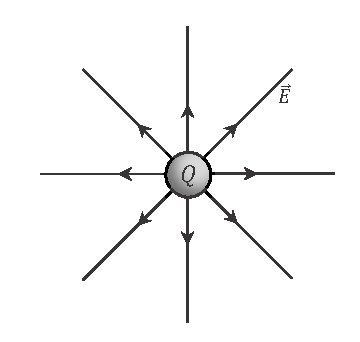
\includegraphics{potential_intro/activity_5_figs/point_charge_E_field.eps}
\end{center}

%\newpage
%\pagebreak[4]
\item The drawing below shows a region of uniform electric field.  Draw a qualitative graph of $V(x)$ along the dotted line shown, defining the potential at point B to be $V=0$.  To check your answer, compare your graph with those you drew in Activity 2.  \label{part_potential_intro_draw_V} 

\begin{center}
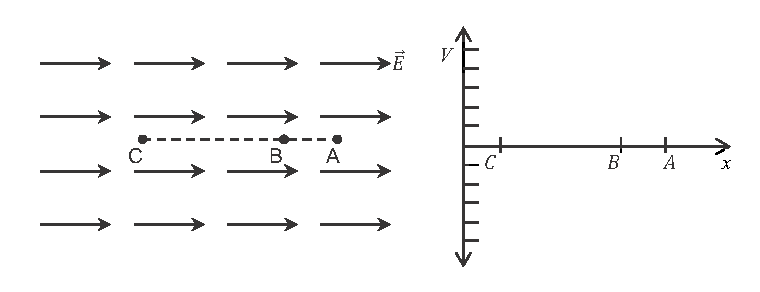
\includegraphics{potential_intro/activity_5_figs/uniform_E_field_3.eps}
\hspace{0.5in}
\begin{lab_axis}[lab_noticks_2quads,
	algebraic_labels,
	width={1.7in}, height={1.6in},
	xlabel={$x$},
	ylabel={$V$},
	xtick={0.2, 0.6, 0.8},
	xticklabels = {C, B, A},
	]
\end{lab_axis}
\end{center}


\end{enumerate}

\textbf{Activity 5: The Electric Potential of a Point Charge}

In part \ref{part_potential_intro_draw_V} of the previous activity, you essentially found $V$ by integrating the electric field, using
$$V=-\int{\vv{E} \cdot \vv{ds}}.$$
Now let's apply this same relationship to one of the most common situations you've seen so far: a single point charge.  We'll put a positive point charge $+Q$ at the origin, at $r=0$, and find the electric potential $V(r)$ due to that point charge.
\begin{center}
\vspace{-0.1 in}
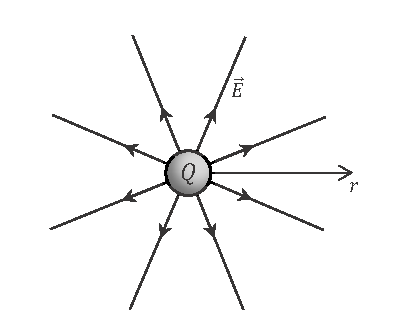
\includegraphics{potential_intro/activity_6_figs/point_charge_E_field_axis.eps}
\end{center}

\begin{enumerate}[labparts]

\item Before we do any calculations, we'll try to get a general feel for what $V(r)$ should look like.  Imagine taking a small charge $q$ out of your pocket, and pushing it in towards $r=0$ from $r=\infty$.  (We'll assume $q$ is positive, so that $U$ and $V$ have the same sign.)  As you push $q$ inward with your hand, does the electric potential due to $Q$ \textit{increase}, \textit{decrease}, or \textit{stay the same} as you get closer to $Q$?
\answerspace{0.4in}

\item The electric field from $Q$ gets stronger as you get closer.  Bearing in mind that $E = -dV/dr$, is the magnitude $\left | {dV}/{dr}\right |$ getting bigger or smaller as you get closer to $Q$?
\answerspace{0.4in}

\item Based on your last two answers, sketch a qualitative graph of $V(r)$ on the axes below.  For convenience, let $V=0$ at $r \rightarrow \infty$. \label{part_potential_intro_sketch_of_Vr}
%\begin{center}
%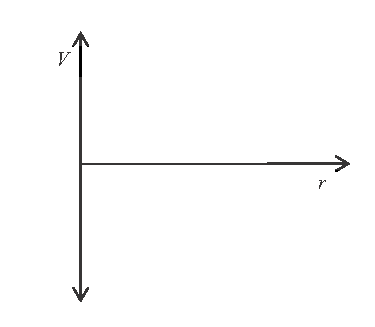
\includegraphics{potential_intro/activity_6_figs/V_axes.eps}
%\end{center}
\begin{lab_axis}*[lab_noticks_2quads,
	width={2.2in}, height={1.9in},
	algebraic_labels,
	xlabel={$r$},
	ylabel={$V$},
	]
\end{lab_axis}

\pagebreak[2]
\item Now that we have some intuition about what $V(r)$ should look like, let's actually do the calculation.  First, write the electric field $E(r)$ at a distance $r$ from the charge in terms of $Q$, $r$, and the Coulomb constant $k_e$.
\answerspace{0.5in}

\item Since the $\vv{E}$ points radially outward, the equation $V=-\int{\vv{E} \cdot \vv{ds}}$ can be reduced to 
the one-dimensional form $V=-\int{E \, dr}$.  Perform that integration to find $V(r)$, using the $E(r)$ you just wrote. Be sure to include an integration constant $+C$.
\answerspace{1.2in}

\item As with the potential energy $U$, you're free to set $C$ to whatever value you want, since the only \textit{physical} meaning of $V$ comes when we take the difference $\Delta V$ between two points.  It's often convenient to set our ``reference value'' of $V$ so that $V=0$ at $r \rightarrow \infty$.  What value of $C$ makes that true?
\answerspace{0.5in}

\item Does your answer for $V(r)$ match with your graph from part \ref{part_potential_intro_sketch_of_Vr}?
\answerspace{0.5in}

%\item draw E(x) along x-axis.  (signs)  Note: save this for the second electric potential lab.

%\item draw V(x) along x-axis.  Check that E = -dV/ds.

\end{enumerate}

You should have found that the electric potential $V$ for a point charge $Q$ is given by
$$V=\frac{k_eQ}{r},$$
where $k_e$ is the Coulomb constant.  The form looks very similar to that of the electric field for a point charge, $E={k_eQ}/{r^2}$, and quick pencil sketches of the two functions tend to look identical.  But of course the two don't have the same units, and the \textit{meaning} of $\vv{E}$ and $V$ are very different---just as distinct as their analogs, $\vv{F}$ and $U$.  
  



